\documentclass[12pt,letterpaper]{article}
\usepackage{graphicx,textcomp}
\usepackage{natbib}
\usepackage{setspace}
\usepackage{fullpage}
\usepackage{color}
\usepackage[reqno]{amsmath}
\usepackage{amsthm}
\usepackage{fancyvrb}
\usepackage{amssymb,enumerate}
\usepackage[all]{xy}
\usepackage{endnotes}
\usepackage{lscape}
\newtheorem{com}{Comment}
\usepackage{float}
\usepackage{hyperref}
\newtheorem{lem} {Lemma}
\newtheorem{prop}{Proposition}
\newtheorem{thm}{Theorem}
\newtheorem{defn}{Definition}
\newtheorem{cor}{Corollary}
\newtheorem{obs}{Observation}
\usepackage[compact]{titlesec}
\usepackage{dcolumn}
\usepackage{tikz}
\usetikzlibrary{arrows}
\usepackage{multirow}
\usepackage{xcolor}
\newcolumntype{.}{D{.}{.}{-1}}
\newcolumntype{d}[1]{D{.}{.}{#1}}
\definecolor{light-gray}{gray}{0.65}
\usepackage{url}
\usepackage{listings}
\usepackage{color}

\definecolor{codegreen}{rgb}{0,0.6,0}
\definecolor{codegray}{rgb}{0.5,0.5,0.5}
\definecolor{codepurple}{rgb}{0.58,0,0.82}
\definecolor{backcolour}{rgb}{0.95,0.95,0.92}

\lstdefinestyle{mystyle}{
	backgroundcolor=\color{backcolour},   
	commentstyle=\color{codegreen},
	keywordstyle=\color{magenta},
	numberstyle=\tiny\color{codegray},
	stringstyle=\color{codepurple},
	basicstyle=\footnotesize,
	breakatwhitespace=false,         
	breaklines=true,                 
	captionpos=b,                    
	keepspaces=true,                 
	numbers=left,                    
	numbersep=5pt,                  
	showspaces=false,                
	showstringspaces=false,
	showtabs=false,                  
	tabsize=2
}
\lstset{style=mystyle}
\newcommand{\Sref}[1]{Section~\ref{#1}}
\newtheorem{hyp}{Hypothesis}

\title{Problem Set 3}
\date{Due: November 12, 2026}
\author{Applied Stats/Quant Methods 1}


\begin{document}
	\maketitle
	\section*{Instructions}
	\begin{itemize}
		\item Please show your work! You may lose points by simply writing in the answer. If the problem requires you to execute commands in \texttt{R}, please include the code you used to get your answers. Please also include the \texttt{.R} file that contains your code. If you are not sure if work needs to be shown for a particular problem, please ask.
	\item Your homework should be submitted electronically on GitHub.
	\item This problem set is due before 23:59 on Thursday November 12, 2026. No late assignments will be accepted.

	\end{itemize}

		\vspace{.25cm}
	
\noindent In this problem set, you will run several regressions and create an add variable plot (see the lecture slides) in \texttt{R} using the \texttt{incumbents\_subset.csv} dataset. Include all of your code.

	\vspace{.5cm}
\section*{Question 1}
\vspace{.25cm}
\noindent We are interested in knowing how the difference in campaign spending between incumbent and challenger affects the incumbent's vote share. 
	\begin{enumerate}
		\item Run a regression where the outcome variable is \texttt{voteshare} and the explanatory variable is \texttt{difflog}.	\vspace{.5cm}
		
		I run a regression using the lm function in .R, and display the results obtained via summary below in Table 1 using the stargazer package. This allows me to access the regression coefficients. The y-intercept, 0.579, is the average vote share of the incumbent expected when the difference in spending is 0. Every one unit increase in the difference in spending is associated, on average, with an increase in vote share of the incumbent of 0.042. 
		\vspace{.5cm}
			\lstinputlisting[language=R, firstline=39, lastline=40]{PS03_answer_ED.R}
			\begin{table}[!htbp] \centering 
				\caption{} 
				\label{} 
				\begin{tabular}{@{\extracolsep{5pt}}lc} 
					\\[-1.8ex]\hline 
					\hline \\[-1.8ex] 
					& \multicolumn{1}{c}{\textit{Dependent variable:}} \\ 
					\cline{2-2} 
					\\[-1.8ex] & voteshare \\ 
					\hline \\[-1.8ex] 
					difflog & 0.042$^{***}$ \\ 
					& (0.001) \\ 
					& \\ 
					Constant & 0.579$^{***}$ \\ 
					& (0.002) \\ 
					& \\ 
					\hline \\[-1.8ex] 
					Observations & 3,193 \\ 
					R$^{2}$ & 0.367 \\ 
					Adjusted R$^{2}$ & 0.367 \\ 
					Residual Std. Error & 0.079 (df = 3191) \\ 
					F Statistic & 1,852.791$^{***}$ (df = 1; 3191) \\ 
					\hline 
					\hline \\[-1.8ex] 
					\textit{Note:}  & \multicolumn{1}{r}{$^{*}$p$<$0.1; $^{**}$p$<$0.05; $^{***}$p$<$0.01} \\ 
				\end{tabular} 
			\end{table} 
			
			
\vspace{2cm}

		\item Make a scatterplot of the two variables and add the regression line. 	\vspace{.25cm}
		
				When examining the relationship between two or more variables, it is useful to employ a visualization tool first, such as a scatterplot. This allows for a first impression even when a regression line is not yet present. 
				
				Below, the scatterplot displays the association between the two variables examined in the regression. The distribution of data points along the regression line indicates a positive linear correlation between the vote share of the incumbent (voteshare) and difference in campaign spending (difflog). 
				
				\vspace{.5cm}
				
				First, the .R code is displayed:
		\lstinputlisting[language=R, firstline=46, lastline=50]{PS03_answer_ED.R}
		
		Th visualization through the scatterplot follows on the next page.
		\begin{center}
		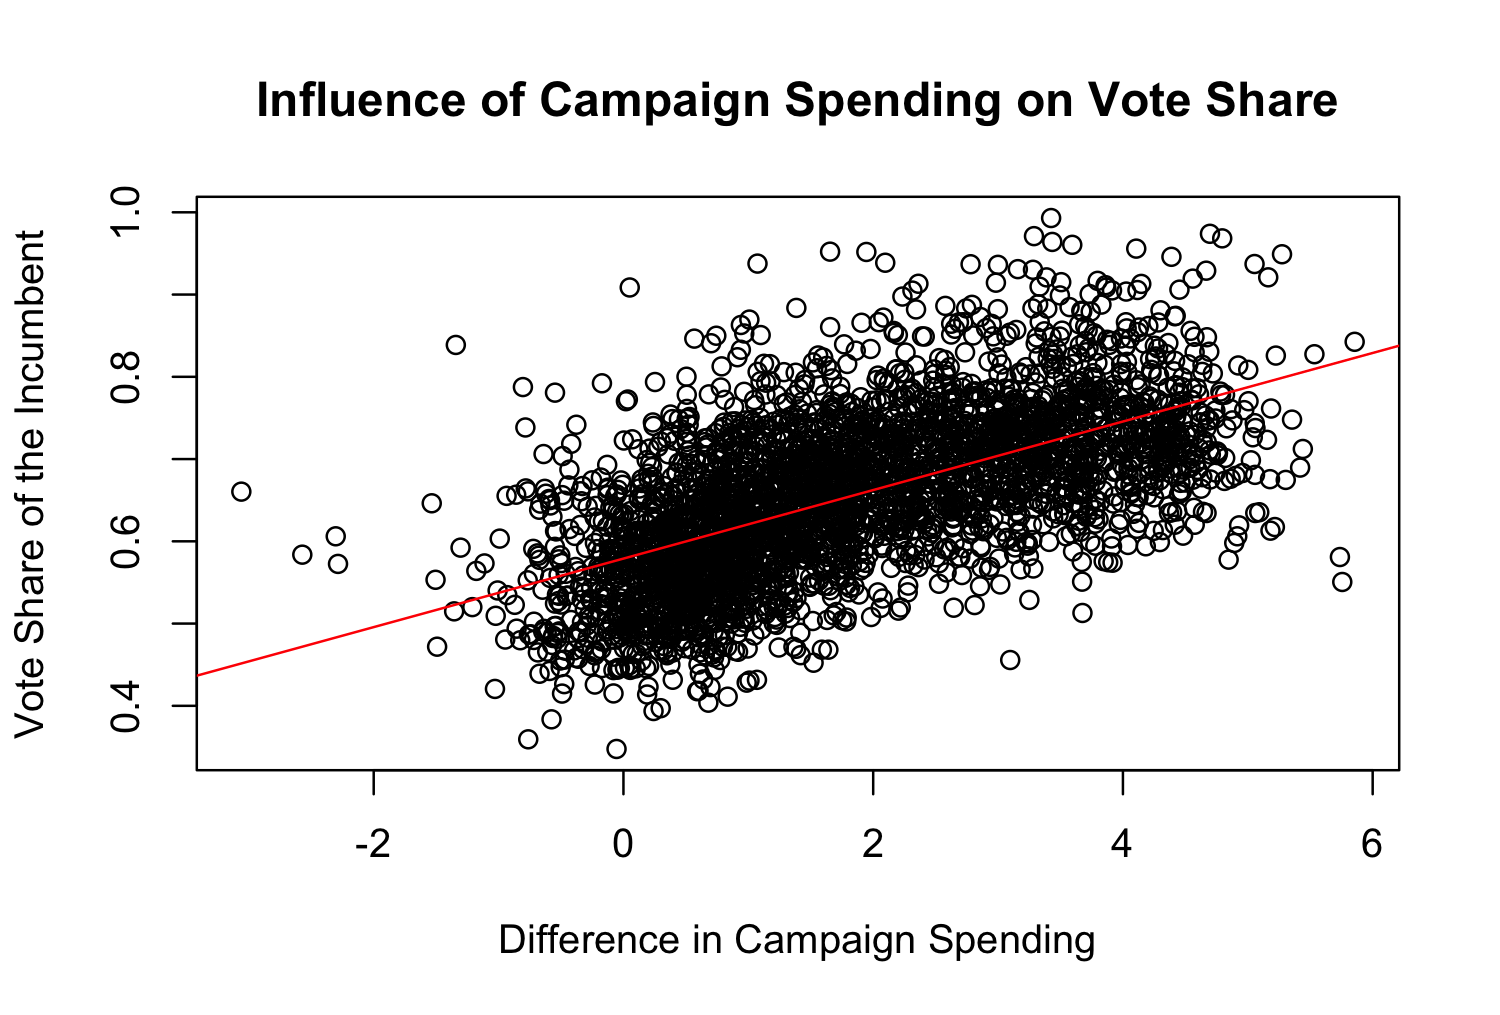
\includegraphics[width=0.8\columnwidth]{PS03_plot1.png}
		\end{center}
		
		\vspace{1cm}
		\item Save the residuals of the model in a separate object.	\vspace{.5cm}
		
		The residuals capture the variation that is not explained by the model. Saving the residuals in a separate object allows for a regression that controls for the explanatory variable difflog to be run later. 
		
		\lstinputlisting[language=R, firstline=54, lastline=55]{PS03_answer_ED.R}
		Table 2 displays the first 6 values of the residuals:
		\begin{table}[!htbp] \centering 
			\caption{} 
			\label{} 
			\begin{tabular}{@{\extracolsep{5pt}} cccccc} 
				\\[-1.8ex]\hline 
				\hline \\[-1.8ex] 
				1 & 2 & 3 & 4 & 5 & 6 \\ 
				\hline \\[-1.8ex] 
				$$-$0.0004$ & $$-$0.032$ & $$-$0.005$ & $0.039$ & $0.036$ & $0.032$ \\ 
				\hline \\[-1.8ex] 
			\end{tabular} 
		\end{table} 
		
		\item Write the prediction equation.
		\vspace{.5cm}
		
			The regression line obtained through the prediction equation is the best fit line based on the sample data. The prediction equation is obtained by inputting y-intercept and slope values into the formula \^{y} = a + bx, which results in this first regression in the following equation:
		\vspace{.25cm}
		
		 \^{y} = 0.579 + 0.042x \centering
	\end{enumerate}
	
\vspace{.25cm}
\section*{Question 2}
\noindent We are interested in knowing how the difference between incumbent and challenger's spending and the vote share of the presidential candidate of the incumbent's party are related.	\vspace{.25cm}
	\begin{enumerate}
		\item Run a regression where the outcome variable is \texttt{presvote} and the explanatory variable is \texttt{difflog}.	\vspace{.5cm}
		
		As before, I run the regression and display the results in Table 3. The y-intercept, 0.508, is the average vote share of the incumbent presidential candidate expected when the difference in campaign spending between challenger and incumbent is 0. Every one unit increase in the difference in spending is associated, on average, with an increase in vote share of the incumbent presidential candidate of 0.024.
		\lstinputlisting[language=R, firstline=64, lastline=65]{PS03_answer_ED.R}
		\begin{table}[!htbp] \centering 
			\caption{} 
			\label{} 
			\begin{tabular}{@{\extracolsep{5pt}}lc} 
				\\[-1.8ex]\hline 
				\hline \\[-1.8ex] 
				& \multicolumn{1}{c}{\textit{Dependent variable:}} \\ 
				\cline{2-2} 
				\\[-1.8ex] & presvote \\ 
				\hline \\[-1.8ex] 
				difflog & 0.024$^{***}$ \\ 
				& (0.001) \\ 
				& \\ 
				Constant & 0.508$^{***}$ \\ 
				& (0.003) \\ 
				& \\ 
				\hline \\[-1.8ex] 
				Observations & 3,193 \\ 
				R$^{2}$ & 0.088 \\ 
				Adjusted R$^{2}$ & 0.088 \\ 
				Residual Std. Error & 0.110 (df = 3191) \\ 
				F Statistic & 307.715$^{***}$ (df = 1; 3191) \\ 
				\hline 
				\hline \\[-1.8ex] 
				\textit{Note:}  & \multicolumn{1}{r}{$^{*}$p$<$0.1; $^{**}$p$<$0.05; $^{***}$p$<$0.01} \\ 
			\end{tabular} 
		\end{table} 
	
		\item Make a scatterplot of the two variables and add the regression line. 	\vspace{.5cm}
		
		The scatterplot of the two variables below indicates a positive linear correlation between the vote share of the incumbent presidential candidate (presvote) and difference in campaign spending (difflog). 
		\vspace{.5cm}
		\lstinputlisting[language=R, firstline=70, lastline=74]{PS03_answer_ED.R}
\begin{center}
	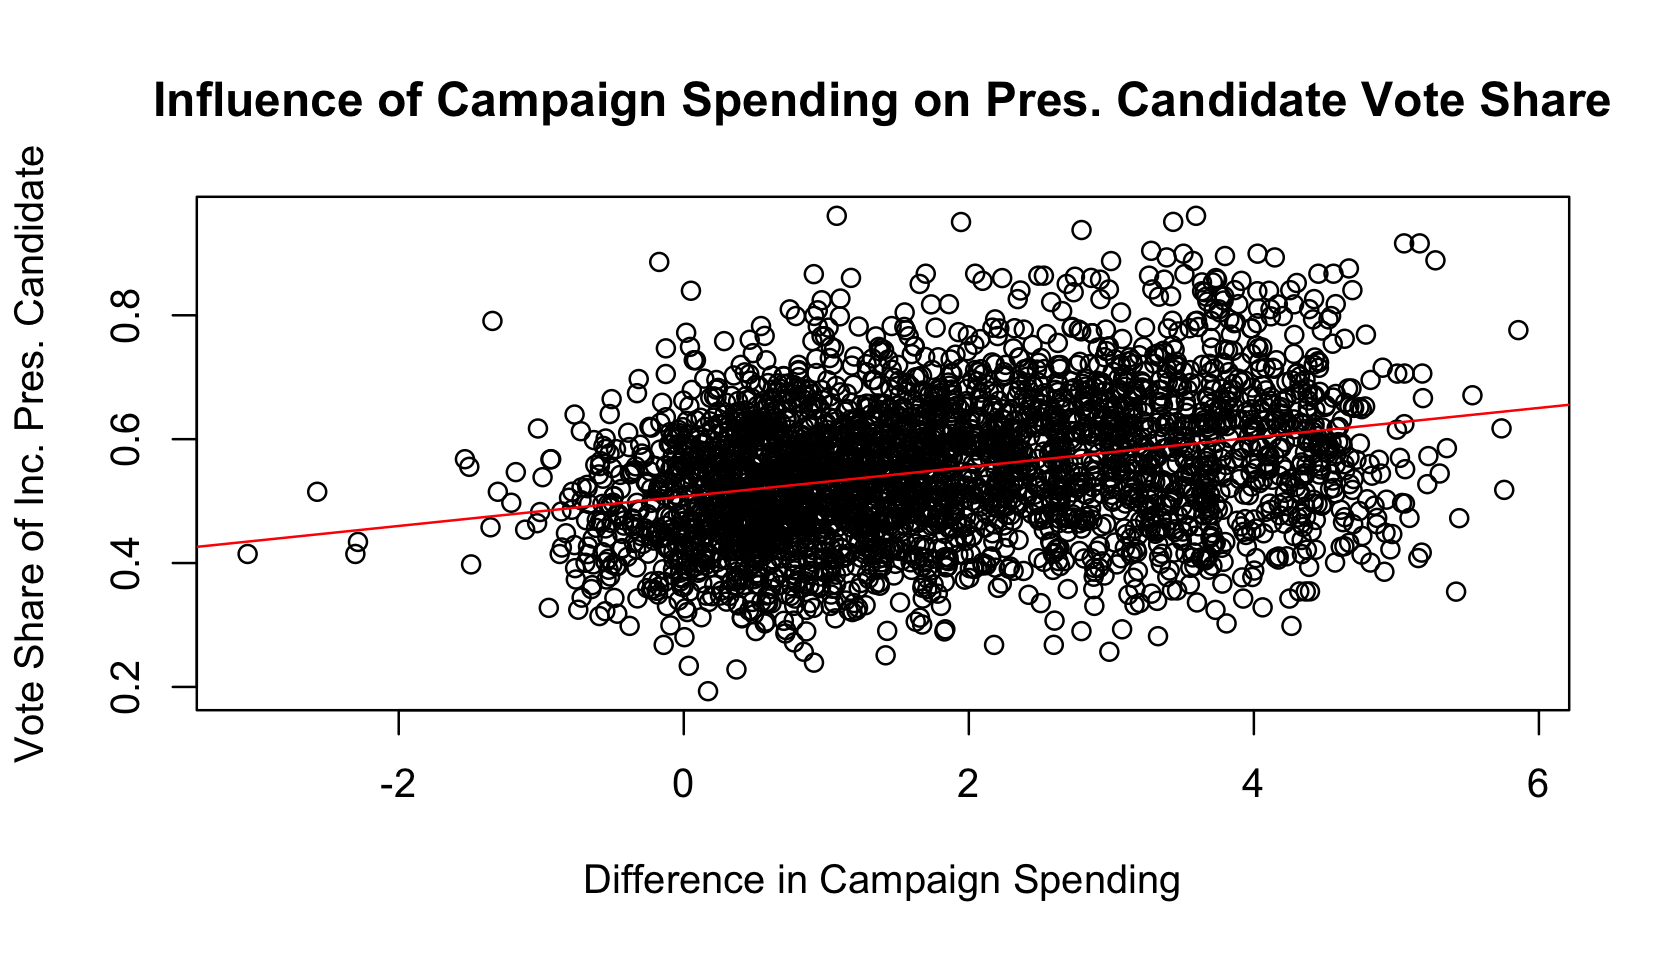
\includegraphics[width=0.8\columnwidth]{PS03_plot2.png}
\end{center}

		\vspace{.2cm}
		\item Save the residuals of the model in a separate object.	\vspace{.5cm}
	
	Saving the residuals in a separate object for this regression allows a regression to be run with the residuals from Question 1, which controls for the explanatory variable difflog. The first 6 values of the residuals of the regression between presvote and difflog are displayed in Table 4.
	\vspace{.5cm}
	\lstinputlisting[language=R, firstline=78, lastline=79]{PS03_answer_ED.R}
	\begin{table}[!htbp] \centering 
		\caption{} 
		\label{} 
		\begin{tabular}{@{\extracolsep{5pt}} cccccc} 
			\\[-1.8ex]\hline 
			\hline \\[-1.8ex] 
			1 & 2 & 3 & 4 & 5 & 6 \\ 
			\hline \\[-1.8ex] 
			$0.006$ & $0.038$ & $$-$0.053$ & $$-$0.053$ & $$-$0.046$ & $0.074$ \\ 
			\hline \\[-1.8ex] 
		\end{tabular} 
	\end{table} 
	
	
		\item Write the prediction equation.
		
		The prediction equation for this model is: \^{y} = 0.508 + 0.024x
	\end{enumerate}
	
	\newpage	
\section*{Question 3}

\noindent We are interested in knowing how the vote share of the presidential candidate of the incumbent's party is associated with the incumbent's electoral success.
	\vspace{.25cm}
	\begin{enumerate}
		\item Run a regression where the outcome variable is \texttt{voteshare} and the explanatory variable is \texttt{presvote}.
			\vspace{.25cm}
			
			Table 5 displays the regression coefficients obtained through the summary of the lm-function. he y-intercept, 0.441, is the average vote share of the incumbent expected when the incumbent presidential candidate's vote share is 0. Every one unit increase in the vote share of the incumbent presidential candidate is associated, on average, with an increase in vote share of the incumbent of 0.388.
			\vspace{.5cm}
			\lstinputlisting[language=R, firstline=88, lastline=89]{PS03_answer_ED.R}
			\begin{table}[!htbp] \centering 
				\caption{} 
				\label{} 
				\begin{tabular}{@{\extracolsep{5pt}}lc} 
					\\[-1.8ex]\hline 
					\hline \\[-1.8ex] 
					& \multicolumn{1}{c}{\textit{Dependent variable:}} \\ 
					\cline{2-2} 
					\\[-1.8ex] & voteshare \\ 
					\hline \\[-1.8ex] 
					presvote & 0.388$^{***}$ \\ 
					& (0.013) \\ 
					& \\ 
					Constant & 0.441$^{***}$ \\ 
					& (0.008) \\ 
					& \\ 
					\hline \\[-1.8ex] 
					Observations & 3,193 \\ 
					R$^{2}$ & 0.206 \\ 
					Adjusted R$^{2}$ & 0.206 \\ 
					Residual Std. Error & 0.088 (df = 3191) \\ 
					F Statistic & 826.950$^{***}$ (df = 1; 3191) \\ 
					\hline 
					\hline \\[-1.8ex] 
					\textit{Note:}  & \multicolumn{1}{r}{$^{*}$p$<$0.1; $^{**}$p$<$0.05; $^{***}$p$<$0.01} \\ 
				\end{tabular} 
			\end{table}
			\newpage
		\item Make a scatterplot of the two variables and add the regression line. 
			\vspace{.5cm}
			
			The scatterplot of the two variables below indicates a positive linear correlation between the vote share of the incumbent party (voteshare) and vote share of the incumbent party's presidential candidate (presvote).
			
			\lstinputlisting[language=R, firstline=94, lastline=98]{PS03_answer_ED.R}
			
\begin{center}
	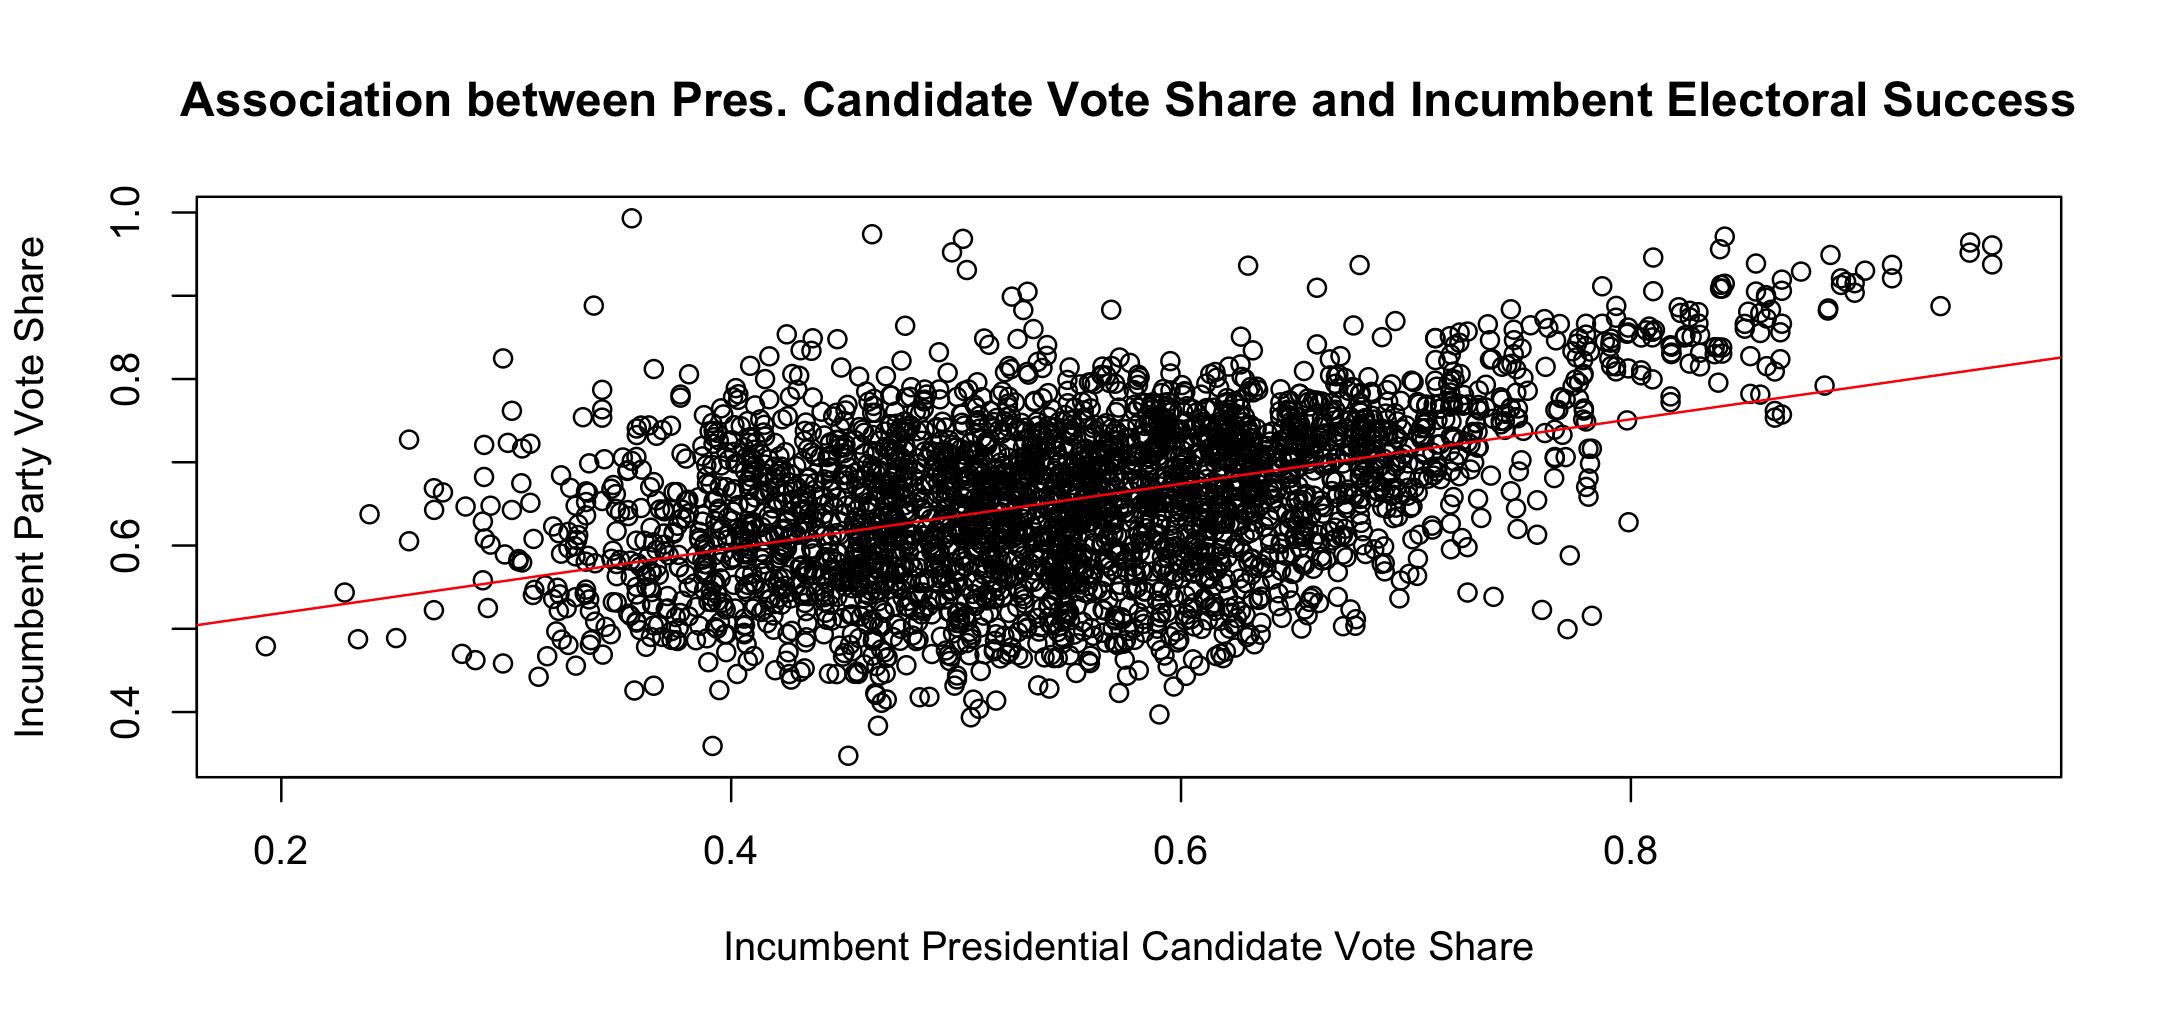
\includegraphics[width=1\columnwidth]{PS03_plot3.png}
\end{center}

		\item Write the prediction equation.
		
		The prediction equation for this model is: \^{y} = 0.441 + 0.388x
	\end{enumerate}
	

\newpage	
\section*{Question 4}
\noindent The residuals from part (a) tell us how much of the variation in \texttt{voteshare} is $not$ explained by the difference in spending between incumbent and challenger. The residuals in part (b) tell us how much of the variation in \texttt{presvote} is $not$ explained by the difference in spending between incumbent and challenger in the district.
	\begin{enumerate}
		\item Run a regression where the outcome variable is the residuals from Question 1 and the explanatory variable is the residuals from Question 2.	\vspace{.5cm}
		
		Below, I now run the regression of the two objects with residuals from Question 1 and 2. This allows us to obtain the regression coefficients displayed in Table 6. The y-intercept is -5.934e-18, displayed in the table as 0.000. The slope is measured to be 0.257. 
		
		\lstinputlisting[language=R, firstline=104, lastline=105]{PS03_answer_ED.R}
		\begin{table}[!htbp] \centering 
			\caption{} 
			\label{} 
			\begin{tabular}{@{\extracolsep{5pt}}lc} 
				\\[-1.8ex]\hline 
				\hline \\[-1.8ex] 
				& \multicolumn{1}{c}{\textit{Dependent variable:}} \\ 
				\cline{2-2} 
				\\[-1.8ex] & model\_1\_res \\ 
				\hline \\[-1.8ex] 
				model\_2\_res & 0.257$^{***}$ \\ 
				& (0.012) \\ 
				& \\ 
				Constant & $-$0.000 \\ 
				& (0.001) \\ 
				& \\ 
				\hline \\[-1.8ex] 
				Observations & 3,193 \\ 
				R$^{2}$ & 0.130 \\ 
				Adjusted R$^{2}$ & 0.130 \\ 
				Residual Std. Error & 0.073 (df = 3191) \\ 
				F Statistic & 476.975$^{***}$ (df = 1; 3191) \\ 
				\hline 
				\hline \\[-1.8ex] 
				\textit{Note:}  & \multicolumn{1}{r}{$^{*}$p$<$0.1; $^{**}$p$<$0.05; $^{***}$p$<$0.01} \\ 
			\end{tabular} 
		\end{table} 
		
		\item Make a scatterplot of the two residuals and add the regression line. 	\vspace{.25cm}
		
		As shown below, the scatterplot displays a positive linear association between the residuasl, that is, the unexplained variation, from the model of incumbent vote share and difference in campaign spending, and the model of incumbent presidential candidate's vote share and difference in campaign spending. 
		
		\lstinputlisting[language=R, firstline=110, lastline=114]{PS03_answer_ED.R}
	\begin{center}
		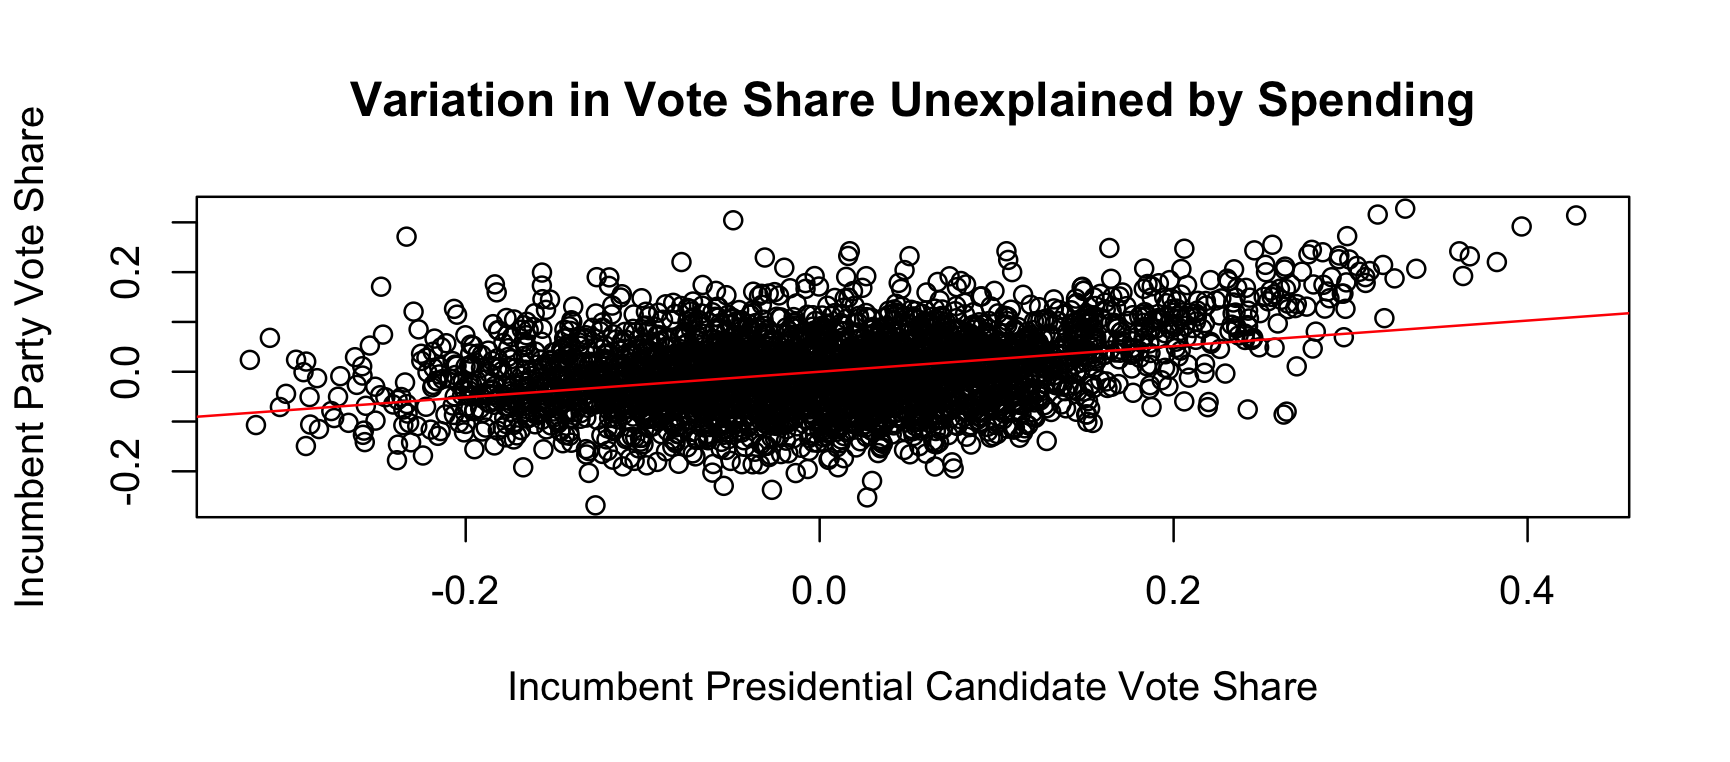
\includegraphics[width=1\columnwidth]{PS03_plot4.png}
	\end{center}
		
		\item Write the prediction equation.
		
		The prediction equation for the regression of the residuals of Questions 1 and 2 is: 
		
		\^{y} = -5.934e-18 + 0.257 \centering
	\end{enumerate}
	
	\newpage	

\section*{Question 5}
\noindent What if the incumbent's vote share is affected by both the president's popularity and the difference in spending between incumbent and challenger? 
	\begin{enumerate}
		\item Run a regression where the outcome variable is the incumbent's \texttt{voteshare} and the explanatory variables are \texttt{difflog} and \texttt{presvote}.	\vspace{.5cm}
		
		Lastly, the multivariate regression displaying the association between the incumbent's vote share and the difference in campaign spending, as well as the vote share of the presidential candidate is run. Table 7 displays the regression coefficients. When the difference in campaign spending and the incumbent presidential candidate's vote share are 0, the vote share of the incumbent party is 0.449. With every one unit increase in the difference in campaign spending, the vote share is increased by 0.036, while with every one unit increase in the incumbent presidential candidate's vote share, the incumbent party's vote share is increased by 0.257.
		
		\lstinputlisting[language=R, firstline=122, lastline=123]{PS03_answer_ED.R}
		\begin{table}[!htbp] \centering 
			\caption{} 
			\label{} 
			\begin{tabular}{@{\extracolsep{5pt}}lc} 
				\\[-1.8ex]\hline 
				\hline \\[-1.8ex] 
				& \multicolumn{1}{c}{\textit{Dependent variable:}} \\ 
				\cline{2-2} 
				\\[-1.8ex] & voteshare \\ 
				\hline \\[-1.8ex] 
				difflog & 0.036$^{***}$ \\ 
				& (0.001) \\ 
				& \\ 
				presvote & 0.257$^{***}$ \\ 
				& (0.012) \\ 
				& \\ 
				Constant & 0.449$^{***}$ \\ 
				& (0.006) \\ 
				& \\ 
				\hline \\[-1.8ex] 
				Observations & 3,193 \\ 
				R$^{2}$ & 0.450 \\ 
				Adjusted R$^{2}$ & 0.449 \\ 
				Residual Std. Error & 0.073 (df = 3190) \\ 
				F Statistic & 1,302.947$^{***}$ (df = 2; 3190) \\ 
				\hline 
				\hline \\[-1.8ex] 
				\textit{Note:}  & \multicolumn{1}{r}{$^{*}$p$<$0.1; $^{**}$p$<$0.05; $^{***}$p$<$0.01} \\ 
			\end{tabular} 
		\end{table} 
		\newpage
		
		\item Write the prediction equation.	\vspace{.5cm}
		
		The prediction equation for this regression is: \^{y} = 0.449 + 0.036$x_1$ + 0.257$x_2$
		\vspace{1cm}
		\item What is it in this output that is identical to the output in Question 4? Why do you think this is the case?
		\vspace{.5cm}
		
		The coefficients for the incumbent presidential candidate's vote share are identical in the models of Question 4 and Question 5. This is because the regression model in Q4 controls for the effect of difference in campaign spending by regressing the residuals of the models of Question 1 and Question 2. As the effect of the difference in campaign spending has been removed from the model in Question 4, we can compute the effect of the incumbent presidential candidate's vote share on the vote share of the party. Hence, the estimated $\beta_2$ coefficient for the incumbent presidential candidate's vote share that is displayed in the output of the multivariate regression is identical to the estimated $\beta_1$ of the model of the residuals that presents the effect of presidential candidate vote share by controlling for difference in campaign spending.
		
	\end{enumerate}




\end{document}
